\DocumentMetadata{
    testphase={phase-III}, % enables tagging
    pdfstandard=A-2b     % declares that the pdf supports the A-2b standard
}

\documentclass[12pt]{article}\usepackage[]{graphicx}\usepackage[]{xcolor}
% maxwidth is the original width if it is less than linewidth
% otherwise use linewidth (to make sure the graphics do not exceed the margin)
\makeatletter
\def\maxwidth{ %
  \ifdim\Gin@nat@width>\linewidth
    \linewidth
  \else
    \Gin@nat@width
  \fi
}
\makeatother

\definecolor{fgcolor}{rgb}{0.345, 0.345, 0.345}
\newcommand{\hlnum}[1]{\textcolor[rgb]{0.686,0.059,0.569}{#1}}%
\newcommand{\hlsng}[1]{\textcolor[rgb]{0.192,0.494,0.8}{#1}}%
\newcommand{\hlcom}[1]{\textcolor[rgb]{0.678,0.584,0.686}{\textit{#1}}}%
\newcommand{\hlopt}[1]{\textcolor[rgb]{0,0,0}{#1}}%
\newcommand{\hldef}[1]{\textcolor[rgb]{0.345,0.345,0.345}{#1}}%
\newcommand{\hlkwa}[1]{\textcolor[rgb]{0.161,0.373,0.58}{\textbf{#1}}}%
\newcommand{\hlkwb}[1]{\textcolor[rgb]{0.69,0.353,0.396}{#1}}%
\newcommand{\hlkwc}[1]{\textcolor[rgb]{0.333,0.667,0.333}{#1}}%
\newcommand{\hlkwd}[1]{\textcolor[rgb]{0.737,0.353,0.396}{\textbf{#1}}}%
\let\hlipl\hlkwb

\usepackage{framed}
\makeatletter
\newenvironment{kframe}{%
 \def\at@end@of@kframe{}%
 \ifinner\ifhmode%
  \def\at@end@of@kframe{\end{minipage}}%
  \begin{minipage}{\columnwidth}%
 \fi\fi%
 \def\FrameCommand##1{\hskip\@totalleftmargin \hskip-\fboxsep
 \colorbox{shadecolor}{##1}\hskip-\fboxsep
     % There is no \\@totalrightmargin, so:
     \hskip-\linewidth \hskip-\@totalleftmargin \hskip\columnwidth}%
 \MakeFramed {\advance\hsize-\width
   \@totalleftmargin\z@ \linewidth\hsize
   \@setminipage}}%
 {\par\unskip\endMakeFramed%
 \at@end@of@kframe}
\makeatother

\definecolor{shadecolor}{rgb}{.97, .97, .97}
\definecolor{messagecolor}{rgb}{0, 0, 0}
\definecolor{warningcolor}{rgb}{1, 0, 1}
\definecolor{errorcolor}{rgb}{1, 0, 0}
\newenvironment{knitrout}{}{} % an empty environment to be redefined in TeX

\usepackage{alltt}
\usepackage{enumitem,xcolor,amsmath}
\usepackage[hyphens]{url}
\usepackage{hyperref}
\usepackage{geometry}


%%
%% The following code is adapted from screenread.sty
%%
\pagestyle{empty}
\newlength\screenwidth
\newlength\screentextwidth
\newcommand\SetScreen[1]{%
  % Argument #1 is the screen width.
  % Set appropriate layout parameters, with only a little white space
  %   around the text.
  % Note that although pagewidth is set to screenwidth in this macro,
  %   this need not always be the case.
  \setlength\screenwidth{#1}%
  \setlength\screentextwidth{#1}%
  \addtolength\screentextwidth{-1cm}%
  \newgeometry{layoutwidth=\screenwidth,
            textwidth=\screentextwidth,
            layoutheight=500cm,
            textheight=500cm,
            top=0.5cm,
            hcentering=true
  }%
}

%%
%% The following code is adapted from screenread.sty
%%
\AddToHook{shipout/before}[SpecialPage]{%
    \pdfpagewidth=\screenwidth  
    \pdfpageheight=\pagetotal
    \advance\pdfpageheight by 2in
    \advance\pdfpageheight by \topmargin
    \advance\pdfpageheight by \textheight % This and next allow for footnotes
    \advance\pdfpageheight by -\pagegoal
}%

\SetScreen{25cm}

\hypersetup{
    pdflang=en-UK,
    pdftitle={CD705: Lecture Week 5.2},
    pdfauthor={Alexey Chernov}
}

\title{{\normalsize CD705: Statistical Data Analysis with R}\\[1ex]
 Lecture 5.2: Data (Pre-)Processing
}



\author{Alexey Chernov\\
  \texttt{A.Chernov@brighton.ac.uk}
}

\date{4 November 2026}

\newcommand{\alert}[1]{\textcolor{red}{#1}}
\IfFileExists{upquote.sty}{\usepackage{upquote}}{}
\begin{document}

\maketitle

\newpage



\begin{knitrout}
\definecolor{shadecolor}{rgb}{0.969, 0.969, 0.969}\color{fgcolor}\begin{kframe}
{\ttfamily\noindent\color{warningcolor}{\#\# Warning in file(file, "{}rt"{}, encoding = fileEncoding): cannot open file 'titanic2208.csv': No such file or directory}}

{\ttfamily\noindent\bfseries\color{errorcolor}{\#\# Error in `file()`:\\\#\# ! cannot open the connection}}

{\ttfamily\noindent\bfseries\color{errorcolor}{\#\# Error:\\\#\# ! object 'titanic' not found}}

{\ttfamily\noindent\bfseries\color{errorcolor}{\#\# Error:\\\#\# ! object 'titanic' not found}}

{\ttfamily\noindent\bfseries\color{errorcolor}{\#\# Error:\\\#\# ! object 'titanic' not found}}

{\ttfamily\noindent\bfseries\color{errorcolor}{\#\# Error:\\\#\# ! object 'titanic' not found}}

{\ttfamily\noindent\bfseries\color{errorcolor}{\#\# Error:\\\#\# ! object 'titanic' not found}}\end{kframe}
\end{knitrout}


\subsubsection*{What We Do with Data}

  \begin{itemize}
    \item Manipulation
      \begin{itemize}
        \item filter (select a subpopulation)
        \item transform (with one or more variables)
        \item aggregate / summarise
        \item re-order
        \item merge
      \end{itemize} 
    \item Visualisation
    \item Modelling (finding patterns), including statistical modelling
  \end{itemize}
  
  \begin{center} 
    \includegraphics[width=0.9\textwidth,alt={A jocular image on summaries}]{SumYearFeetPopulation.jpg} 
  \end{center} 

\newpage  
\subsubsection*{Contingency Tables}

Contingency tables is a powerful and versatile tool for summarising 
the relationship between several categorical variables.
\begin{knitrout}
\definecolor{shadecolor}{rgb}{0.969, 0.969, 0.969}\color{fgcolor}\begin{kframe}
\begin{alltt}
\hlkwd{with}\hldef{(titanic,}
     \hlkwd{table}\hldef{(Sex,Survived)}
     \hldef{)}
\end{alltt}


{\ttfamily\noindent\bfseries\color{errorcolor}{\#\# Error:\\\#\# ! object 'titanic' not found}}\begin{alltt}
\hlkwd{with}\hldef{(titanic,}
     \hlkwd{table}\hldef{(Sex,Class)}
     \hldef{)}
\end{alltt}


{\ttfamily\noindent\bfseries\color{errorcolor}{\#\# Error:\\\#\# ! object 'titanic' not found}}\begin{alltt}
\hlkwd{with}\hldef{(titanic,}
     \hlkwd{table}\hldef{(Sex,}\hlkwc{Passengers} \hldef{= Class} \hlopt{%in%} \hlkwd{c}\hldef{(}\hlsng{"1st Class"}\hldef{,}\hlsng{"2nd Class"}\hldef{,}\hlsng{"3rd Class"}\hldef{))}
     \hldef{)}
\end{alltt}


{\ttfamily\noindent\bfseries\color{errorcolor}{\#\# Error:\\\#\# ! object 'titanic' not found}}\begin{alltt}
\hlkwd{with}\hldef{(titanic,}
     \hlkwd{table}\hldef{(Sex,Survived,Class)}
     \hldef{)}
\end{alltt}


{\ttfamily\noindent\bfseries\color{errorcolor}{\#\# Error:\\\#\# ! object 'titanic' not found}}\end{kframe}
\end{knitrout}

Proportion tables help replace absolute frequencies by relative ones:
\begin{knitrout}
\definecolor{shadecolor}{rgb}{0.969, 0.969, 0.969}\color{fgcolor}\begin{kframe}
\begin{alltt}
\hlkwd{with}\hldef{(titanic,}
     \hlkwd{table}\hldef{(Sex,Survived)}
     \hldef{)}
\end{alltt}


{\ttfamily\noindent\bfseries\color{errorcolor}{\#\# Error:\\\#\# ! object 'titanic' not found}}\begin{alltt}
\hlkwd{with}\hldef{(titanic,}
     \hlkwd{proportions}\hldef{(}\hlkwd{table}\hldef{(Sex,Survived))}
     \hldef{)}
\end{alltt}


{\ttfamily\noindent\bfseries\color{errorcolor}{\#\# Error:\\\#\# ! object 'titanic' not found}}\begin{alltt}
\hlkwd{with}\hldef{(titanic,}
     \hlkwd{proportions}\hldef{(}\hlkwd{table}\hldef{(Sex,Survived),}\hlkwc{margin}\hldef{=}\hlnum{1}\hldef{)}
     \hldef{)}
\end{alltt}


{\ttfamily\noindent\bfseries\color{errorcolor}{\#\# Error:\\\#\# ! object 'titanic' not found}}\begin{alltt}
\hlkwd{with}\hldef{(titanic,}
     \hlkwd{proportions}\hldef{(}\hlkwd{table}\hldef{(Sex,Survived),}\hlkwc{margin}\hldef{=}\hlnum{2}\hldef{)}
     \hldef{)}
\end{alltt}


{\ttfamily\noindent\bfseries\color{errorcolor}{\#\# Error:\\\#\# ! object 'titanic' not found}}\end{kframe}
\end{knitrout}

Advanced use of tables:
\begin{knitrout}
\definecolor{shadecolor}{rgb}{0.969, 0.969, 0.969}\color{fgcolor}\begin{kframe}
\begin{alltt}
\hlkwd{length}\hldef{(}\hlkwd{unique}\hldef{(titanic}\hlopt{$}\hldef{Name))}
\end{alltt}


{\ttfamily\noindent\bfseries\color{errorcolor}{\#\# Error:\\\#\# ! object 'titanic' not found}}\begin{alltt}
\hldef{repeated.names} \hlkwb{<-} \hlkwd{with}\hldef{(titanic,}
                       \hlkwd{names}\hldef{(}\hlkwd{table}\hldef{(Name)[}\hlkwd{table}\hldef{(Name)}\hlopt{>}\hlnum{1}\hldef{])}
                       \hldef{)}
\end{alltt}


{\ttfamily\noindent\bfseries\color{errorcolor}{\#\# Error:\\\#\# ! object 'titanic' not found}}\begin{alltt}
\hldef{rep.titanic} \hlkwb{<-} \hldef{titanic[titanic}\hlopt{$}\hldef{Name} \hlopt{%in%} \hldef{repeated.names,]}
\end{alltt}


{\ttfamily\noindent\bfseries\color{errorcolor}{\#\# Error:\\\#\# ! object 'titanic' not found}}\begin{alltt}
\hlkwd{with}\hldef{(rep.titanic,}
     \hldef{rep.titanic[}\hlkwd{order}\hldef{(Name,Age.Whole.Years,Joined),}
                 \hlkwd{c}\hldef{(}\hlsng{"Name"}\hldef{,}\hlsng{"Class"}\hldef{,}\hlsng{"Age.Whole.Years"}\hldef{,}\hlsng{"Joined"}\hldef{,}\hlsng{"Survived"}\hldef{)]}
\hldef{)}
\end{alltt}


{\ttfamily\noindent\bfseries\color{errorcolor}{\#\# Error:\\\#\# ! object 'rep.titanic' not found}}\end{kframe}
\end{knitrout}


\newpage  
\subsubsection*{Data Shapes}  

    \begin{center}
     \begin{tabular}[b]{l|c|c|c|}
        & Algebra & English & History \\
      \hline
       Jane & 40 & 57 & 61 \\
      \hline 
       John & 53 & 73 & 39 \\
      \hline 
     \end{tabular}
     %
     \qquad
     %
     \begin{tabular}[b]{l|c|c|}
        & Jane & John \\
      \hline
       Algebra & 40 & 53 \\
      \hline 
       English & 57 & 73 \\
      \hline
       History & 61 & 39 \\
      \hline 
     \end{tabular}
     
     \bigskip
     
     \begin{tabular}[t]{l|l|c}
       Name & Subject & Mark\\
      \hline
       Jane & Algebra & 40\\
       Jane & English & 57 \\
       Jane & History & 61 \\
       John & Algebra & 53\\
       John & English & 73 \\
       John & History & 39 \\
     \end{tabular}
   \end{center}

The two tables at the top are data in the so called ``wide'' format. 
The bottom table is the data in a ``long'' format. 
The latter is often necessary for regression-based statistical methods such as ANOVA but
also useful for data re-shaping.

\begin{knitrout}
\definecolor{shadecolor}{rgb}{0.969, 0.969, 0.969}\color{fgcolor}\begin{kframe}
\begin{alltt}
\hldef{df1} \hlkwb{<-} \hlkwd{data.frame}\hldef{(}\hlkwc{Subject}\hldef{=}\hlkwd{c}\hldef{(}\hlsng{"Algebra"}\hldef{,}\hlsng{"English"}\hldef{,}\hlsng{"History"}\hldef{),}
                  \hlkwc{Jane}\hldef{=}\hlkwd{c}\hldef{(}\hlnum{40}\hldef{,}\hlnum{57}\hldef{,}\hlnum{61}\hldef{),}
                  \hlkwc{John}\hldef{=}\hlkwd{c}\hldef{(}\hlnum{53}\hldef{,}\hlnum{73}\hldef{,}\hlnum{39}\hldef{),}
                  \hlkwc{stringsAsFactors}\hldef{=}\hlnum{TRUE}
                  \hldef{)}
\hldef{df1}
\end{alltt}
\begin{verbatim}
##   Subject Jane John
## 1 Algebra   40   53
## 2 English   57   73
## 3 History   61   39
\end{verbatim}
\end{kframe}
\end{knitrout}

\begin{knitrout}
\definecolor{shadecolor}{rgb}{0.969, 0.969, 0.969}\color{fgcolor}\begin{kframe}
\begin{alltt}
\hlkwd{library}\hldef{(reshape2)}
\end{alltt}


{\ttfamily\noindent\bfseries\color{errorcolor}{\#\# Error in `library()`:\\\#\# ! there is no package called 'reshape2'}}\begin{alltt}
\hldef{df2} \hlkwb{<-} \hlkwd{melt}\hldef{(df1,}\hlkwc{id.vars}\hldef{=}\hlkwd{c}\hldef{(}\hlsng{"Subject"}\hldef{),}
            \hlkwc{measure.vars}\hldef{=}\hlkwd{c}\hldef{(}\hlsng{"Jane"}\hldef{,}\hlsng{"John"}\hldef{),}
            \hlkwc{variable.name}\hldef{=}\hlsng{"Name"}\hldef{,}
            \hlkwc{value.name}\hldef{=}\hlsng{"Mark"}\hldef{)}
\end{alltt}


{\ttfamily\noindent\bfseries\color{errorcolor}{\#\# Error in `melt()`:\\\#\# ! could not find function "{}melt"{}}}\begin{alltt}
\hldef{df2}
\end{alltt}


{\ttfamily\noindent\bfseries\color{errorcolor}{\#\# Error:\\\#\# ! object 'df2' not found}}\begin{alltt}
\hldef{df2} \hlkwb{<-} \hldef{df2[,}\hlkwd{c}\hldef{(}\hlsng{"Name"}\hldef{,}\hlsng{"Subject"}\hldef{,}\hlsng{"Mark"}\hldef{)]}
\end{alltt}


{\ttfamily\noindent\bfseries\color{errorcolor}{\#\# Error:\\\#\# ! object 'df2' not found}}\begin{alltt}
\hldef{df2}
\end{alltt}


{\ttfamily\noindent\bfseries\color{errorcolor}{\#\# Error:\\\#\# ! object 'df2' not found}}\end{kframe}
\end{knitrout}

\begin{knitrout}
\definecolor{shadecolor}{rgb}{0.969, 0.969, 0.969}\color{fgcolor}\begin{kframe}
\begin{alltt}
\hldef{df1a} \hlkwb{<-} \hlkwd{dcast}\hldef{(df2,Subject}\hlopt{~}\hldef{Name,}\hlkwc{value.var}\hldef{=}\hlsng{"Mark"}\hldef{)}
\end{alltt}


{\ttfamily\noindent\bfseries\color{errorcolor}{\#\# Error in `dcast()`:\\\#\# ! could not find function "{}dcast"{}}}\begin{alltt}
\hldef{df1a}
\end{alltt}


{\ttfamily\noindent\bfseries\color{errorcolor}{\#\# Error:\\\#\# ! object 'df1a' not found}}\end{kframe}
\end{knitrout}

\begin{knitrout}
\definecolor{shadecolor}{rgb}{0.969, 0.969, 0.969}\color{fgcolor}\begin{kframe}
\begin{alltt}
\hldef{df3} \hlkwb{<-} \hlkwd{dcast}\hldef{(df2,Name}\hlopt{~}\hldef{Subject,}\hlkwc{value.var}\hldef{=}\hlsng{"Mark"}\hldef{)}
\end{alltt}


{\ttfamily\noindent\bfseries\color{errorcolor}{\#\# Error in `dcast()`:\\\#\# ! could not find function "{}dcast"{}}}\begin{alltt}
\hldef{df3}
\end{alltt}


{\ttfamily\noindent\bfseries\color{errorcolor}{\#\# Error:\\\#\# ! object 'df3' not found}}\end{kframe}
\end{knitrout}

Read \textit{Tidy Data} by Hadley Wickham!

\subsubsection*{Experimental Data}

In experiments, we measure a response in some subjects to a range of conditions  

    \begin{center}
     \begin{tabular}[t]{c|c|c}
       \multicolumn{3}{c}{Wide format}\\[1ex]
       Subject & Condition A & Condition B \\
      \hline
       1 & \(0.3007\) & \(0.9286\) \\
       2 & \(-1.0123\) & \(-0.8614\) \\
       3 & \(0.5813\) & \(0.7814\) \\
     \end{tabular}
     %
     \qquad
     %
     \begin{tabular}[t]{c|c|c}
       \multicolumn{3}{c}{Long format}\\[1ex]
       Subject & Condition & Response\\
      \hline
       1 & A & \(0.3007\)\\
       1 & B & \(0.9286\) \\
       2 & A & \(-1.0123\) \\
       2 & B & \(-0.8614\) \\
       3 & A & \(0.5813\) \\ 
       3 & B & \(0.7814\)\\
     \end{tabular}
   \end{center}

 We look for a rule: \(\text{Response} \sim \text{Condition(s)}\)  

\subsubsection*{Splits and Merges}
\begin{knitrout}
\definecolor{shadecolor}{rgb}{0.969, 0.969, 0.969}\color{fgcolor}\begin{kframe}
\begin{alltt}
\hldef{(df.girls} \hlkwb{<-} \hldef{df3[df3}\hlopt{$}\hldef{Name}\hlopt{==}\hlsng{"Jane"}\hldef{,])}
\end{alltt}


{\ttfamily\noindent\bfseries\color{errorcolor}{\#\# Error:\\\#\# ! object 'df3' not found}}\begin{alltt}
\hldef{(df.boys} \hlkwb{<-} \hldef{df3[df3}\hlopt{$}\hldef{Name}\hlopt{==}\hlsng{"John"}\hldef{,])}
\end{alltt}


{\ttfamily\noindent\bfseries\color{errorcolor}{\#\# Error:\\\#\# ! object 'df3' not found}}\begin{alltt}
\hlkwd{rownames}\hldef{(df.boys)}\hlkwb{<-}\hlkwa{NULL}
\end{alltt}


{\ttfamily\noindent\bfseries\color{errorcolor}{\#\# Error:\\\#\# ! object 'df.boys' not found}}\begin{alltt}
\hldef{df.boys}
\end{alltt}


{\ttfamily\noindent\bfseries\color{errorcolor}{\#\# Error:\\\#\# ! object 'df.boys' not found}}\end{kframe}
\end{knitrout}

\begin{knitrout}
\definecolor{shadecolor}{rgb}{0.969, 0.969, 0.969}\color{fgcolor}\begin{kframe}
\begin{alltt}
\hlkwd{rbind}\hldef{(df.girls,df.boys)}
\end{alltt}


{\ttfamily\noindent\bfseries\color{errorcolor}{\#\# Error:\\\#\# ! object 'df.girls' not found}}\end{kframe}
\end{knitrout}

\begin{knitrout}
\definecolor{shadecolor}{rgb}{0.969, 0.969, 0.969}\color{fgcolor}\begin{kframe}
\begin{alltt}
\hldef{(df.girls.vars} \hlkwb{<-} \hldef{df1[,}\hlopt{!}\hldef{(}\hlkwd{names}\hldef{(df1)} \hlopt{%in%} \hlkwd{c}\hldef{(}\hlsng{"John"}\hldef{))])}
\end{alltt}
\begin{verbatim}
##   Subject Jane
## 1 Algebra   40
## 2 English   57
## 3 History   61
\end{verbatim}
\begin{alltt}
\hldef{(df.boys.vars} \hlkwb{<-} \hldef{df1[,}\hlopt{-}\hlnum{2}\hldef{])}
\end{alltt}
\begin{verbatim}
##   Subject John
## 1 Algebra   53
## 2 English   73
## 3 History   39
\end{verbatim}
\end{kframe}
\end{knitrout}

\begin{knitrout}
\definecolor{shadecolor}{rgb}{0.969, 0.969, 0.969}\color{fgcolor}\begin{kframe}
\begin{alltt}
\hlkwd{merge}\hldef{(df.girls.vars,df.boys.vars)}
\end{alltt}
\begin{verbatim}
##   Subject Jane John
## 1 Algebra   40   53
## 2 English   57   73
## 3 History   61   39
\end{verbatim}
\end{kframe}
\end{knitrout}

\subsubsection*{Missing Values and Outliers}

An important part of pre-processing is dealing with missing values and 
outliers (unusual observations).
Outliers may be more dangerous as they are not normally marked as such.
Missing values may also have unusual and non-obvious encodings.

Both missing values and outliers may be systematic or random. 
The stratedy for dealing with them must depend on their origin.

\bigskip

Strategies to deal with missing values (and outliers):
\begin{itemize}
  \item case-by-case (for each operation separately);
  \item remove an observation;
  \item remove a variable;
  \item imputation:
    \begin{itemize}
      \item fundamental (collecting the data element again);
      \item technical: by average, by function of other variable(s), 
        by a stochastic procedure. 
    \end{itemize}
\end{itemize}

\newpage
\subsection*{Data Modelling}

Data Modelling includes finding any patterns or regularities in data.
Typically, it assumes comparing the data with some theoretical expectation.
The latter depends on the business context and changes while the data are analysed. 

Any data set can be considered as a selection from a large population.
Two kinds of selection methods:
\begin{itemize}
  \item observational (sampling-based);
  \item experimental.
\end{itemize}
The involved randomness may be natural or imposed by us.

\subsubsection*{Hypothesis Testing}

Is the number of men and women approximately equal in the 1st Class?
\begin{knitrout}
\definecolor{shadecolor}{rgb}{0.969, 0.969, 0.969}\color{fgcolor}\begin{kframe}
\begin{alltt}
\hlkwd{attach}\hldef{(titanic)}
\end{alltt}


{\ttfamily\noindent\bfseries\color{errorcolor}{\#\# Error:\\\#\# ! object 'titanic' not found}}\begin{alltt}
\hldef{(Sexes} \hlkwb{<-} \hlkwd{table}\hldef{(Sex[Class}\hlopt{==}\hlsng{"1st Class"}\hldef{]))}
\end{alltt}


{\ttfamily\noindent\bfseries\color{errorcolor}{\#\# Error:\\\#\# ! object 'Sex' not found}}\begin{alltt}
\hlkwd{binom.test}\hldef{(Sexes[}\hlnum{1}\hldef{],}\hlkwd{sum}\hldef{(Sexes))}
\end{alltt}


{\ttfamily\noindent\bfseries\color{errorcolor}{\#\# Error:\\\#\# ! object 'Sexes' not found}}\begin{alltt}
\hlkwd{pbinom}\hldef{(}\hlkwd{min}\hldef{(Sexes),}\hlkwd{sum}\hldef{(Sexes),}\hlnum{0.5}\hldef{)}\hlopt{*}\hlnum{2}
\end{alltt}


{\ttfamily\noindent\bfseries\color{errorcolor}{\#\# Error:\\\#\# ! object 'Sexes' not found}}\begin{alltt}
\hlkwd{detach}\hldef{(titanic)}
\end{alltt}


{\ttfamily\noindent\bfseries\color{errorcolor}{\#\# Error in `detach()`:\\\#\# ! invalid 'name' argument}}\end{kframe}
\end{knitrout}

Are 3rd class and 2nd Class passengers of the same median age?
\begin{knitrout}
\definecolor{shadecolor}{rgb}{0.969, 0.969, 0.969}\color{fgcolor}\begin{kframe}
\begin{alltt}
\hlkwd{attach}\hldef{(titanic)}
\end{alltt}


{\ttfamily\noindent\bfseries\color{errorcolor}{\#\# Error:\\\#\# ! object 'titanic' not found}}\begin{alltt}
\hlkwd{plot}\hldef{(}\hlkwd{density}\hldef{(Age.Whole.Years[Class}\hlopt{==}\hlsng{"3rd Class"}\hldef{],}\hlkwc{na.rm}\hldef{=}\hlnum{TRUE}\hldef{),}\hlkwc{col}\hldef{=}\hlsng{"red"}\hldef{)}
\end{alltt}


{\ttfamily\noindent\bfseries\color{errorcolor}{\#\# Error:\\\#\# ! object 'Age.Whole.Years' not found}}\begin{alltt}
\hlkwd{lines}\hldef{(}\hlkwd{density}\hldef{(Age.Whole.Years[Class}\hlopt{==}\hlsng{"2nd Class"}\hldef{],}\hlkwc{na.rm}\hldef{=}\hlnum{TRUE}\hldef{),}\hlkwc{col}\hldef{=}\hlsng{"blue"}\hldef{)}
\end{alltt}


{\ttfamily\noindent\bfseries\color{errorcolor}{\#\# Error:\\\#\# ! object 'Age.Whole.Years' not found}}\begin{alltt}
\hlkwd{wilcox.test}\hldef{(Age.Whole.Years[Class}\hlopt{==}\hlsng{"3rd Class"}\hldef{],Age.Whole.Years[Class}\hlopt{==}\hlsng{"2nd Class"}\hldef{])}
\end{alltt}


{\ttfamily\noindent\bfseries\color{errorcolor}{\#\# Error:\\\#\# ! object 'Age.Whole.Years' not found}}\begin{alltt}
\hlkwd{detach}\hldef{(titanic)}
\end{alltt}


{\ttfamily\noindent\bfseries\color{errorcolor}{\#\# Error in `detach()`:\\\#\# ! invalid 'name' argument}}\end{kframe}
\end{knitrout}

Did the chance of survival depend on sex?
\begin{knitrout}
\definecolor{shadecolor}{rgb}{0.969, 0.969, 0.969}\color{fgcolor}\begin{kframe}
\begin{alltt}
\hlkwd{attach}\hldef{(titanic)}
\end{alltt}


{\ttfamily\noindent\bfseries\color{errorcolor}{\#\# Error:\\\#\# ! object 'titanic' not found}}\begin{alltt}
\hldef{(SS} \hlkwb{<-} \hlkwd{table}\hldef{(Sex,Survived))}
\end{alltt}


{\ttfamily\noindent\bfseries\color{errorcolor}{\#\# Error:\\\#\# ! object 'Sex' not found}}\begin{alltt}
\hlkwd{fisher.test}\hldef{(SS)}
\end{alltt}


{\ttfamily\noindent\bfseries\color{errorcolor}{\#\# Error:\\\#\# ! object 'SS' not found}}\begin{alltt}
\hlkwd{detach}\hldef{(titanic)}
\end{alltt}


{\ttfamily\noindent\bfseries\color{errorcolor}{\#\# Error in `detach()`:\\\#\# ! invalid 'name' argument}}\end{kframe}
\end{knitrout}

\newpage
\subsubsection*{Linear Regression}

Simple regression (trend line):
\begin{knitrout}
\definecolor{shadecolor}{rgb}{0.969, 0.969, 0.969}\color{fgcolor}\begin{kframe}
\begin{alltt}
\hlkwd{plot}\hldef{(Petal.Length}\hlopt{~}\hldef{Petal.Width,}\hlkwc{data}\hldef{=iris)}
\hldef{PLW} \hlkwb{<-} \hlkwd{lm}\hldef{(Petal.Length}\hlopt{~}\hldef{Petal.Width,}\hlkwc{data}\hldef{=iris)}
\hldef{PLW}
\end{alltt}
\begin{verbatim}
## 
## Call:
## lm(formula = Petal.Length ~ Petal.Width, data = iris)
## 
## Coefficients:
## (Intercept)  Petal.Width  
##       1.084        2.230
\end{verbatim}
\begin{alltt}
\hlkwd{summary}\hldef{(PLW)}
\end{alltt}
\begin{verbatim}
## 
## Call:
## lm(formula = Petal.Length ~ Petal.Width, data = iris)
## 
## Residuals:
##      Min       1Q   Median       3Q      Max 
## -1.33542 -0.30347 -0.02955  0.25776  1.39453 
## 
## Coefficients:
##             Estimate Std. Error t value Pr(>|t|)    
## (Intercept)  1.08356    0.07297   14.85   <2e-16 ***
## Petal.Width  2.22994    0.05140   43.39   <2e-16 ***
## ---
## Signif. codes:  0 '***' 0.001 '**' 0.01 '*' 0.05 '.' 0.1 ' ' 1
## 
## Residual standard error: 0.4782 on 148 degrees of freedom
## Multiple R-squared:  0.9271,	Adjusted R-squared:  0.9266 
## F-statistic:  1882 on 1 and 148 DF,  p-value: < 2.2e-16
\end{verbatim}
\begin{alltt}
\hlkwd{abline}\hldef{(PLW,} \hlkwc{col}\hldef{=}\hlsng{"blue"}\hldef{,}\hlkwc{lwd}\hldef{=}\hlnum{3}\hldef{)}
\end{alltt}
\end{kframe}

{\centering 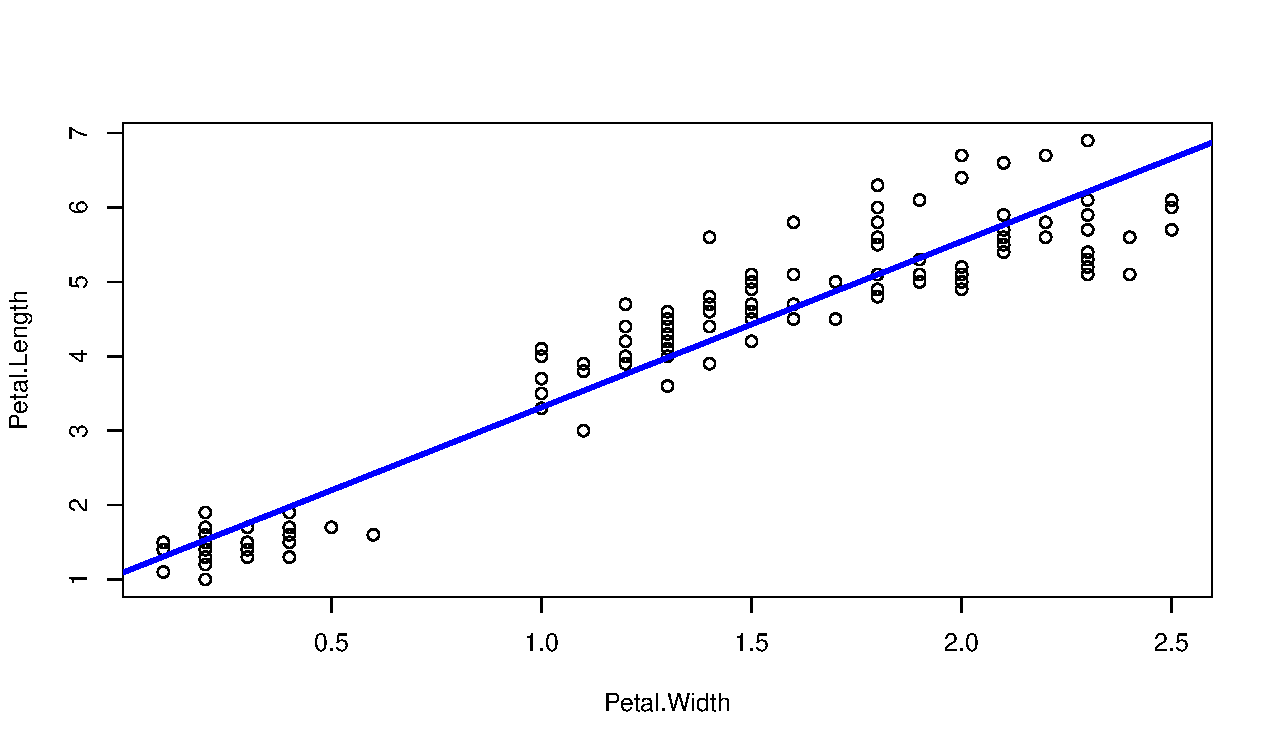
\includegraphics[width=\maxwidth]{figure/iris-Petal.Length-Petal.Width-1} 

}


\end{knitrout}

\begin{knitrout}
\definecolor{shadecolor}{rgb}{0.969, 0.969, 0.969}\color{fgcolor}\begin{kframe}
\begin{alltt}
\hlkwd{plot}\hldef{(Sepal.Length}\hlopt{~}\hldef{Sepal.Width,}\hlkwc{data}\hldef{=iris)}
\hldef{SLW} \hlkwb{<-} \hlkwd{lm}\hldef{(Sepal.Length}\hlopt{~}\hldef{Sepal.Width,}\hlkwc{data}\hldef{=iris)}
\hlkwd{summary}\hldef{(SLW)}
\end{alltt}
\begin{verbatim}
## 
## Call:
## lm(formula = Sepal.Length ~ Sepal.Width, data = iris)
## 
## Residuals:
##     Min      1Q  Median      3Q     Max 
## -1.5561 -0.6333 -0.1120  0.5579  2.2226 
## 
## Coefficients:
##             Estimate Std. Error t value Pr(>|t|)    
## (Intercept)   6.5262     0.4789   13.63   <2e-16 ***
## Sepal.Width  -0.2234     0.1551   -1.44    0.152    
## ---
## Signif. codes:  0 '***' 0.001 '**' 0.01 '*' 0.05 '.' 0.1 ' ' 1
## 
## Residual standard error: 0.8251 on 148 degrees of freedom
## Multiple R-squared:  0.01382,	Adjusted R-squared:  0.007159 
## F-statistic: 2.074 on 1 and 148 DF,  p-value: 0.1519
\end{verbatim}
\begin{alltt}
\hlkwd{abline}\hldef{(SLW,} \hlkwc{col}\hldef{=}\hlsng{"blue"}\hldef{,}\hlkwc{lwd}\hldef{=}\hlnum{3}\hldef{)}
\end{alltt}
\end{kframe}

{\centering 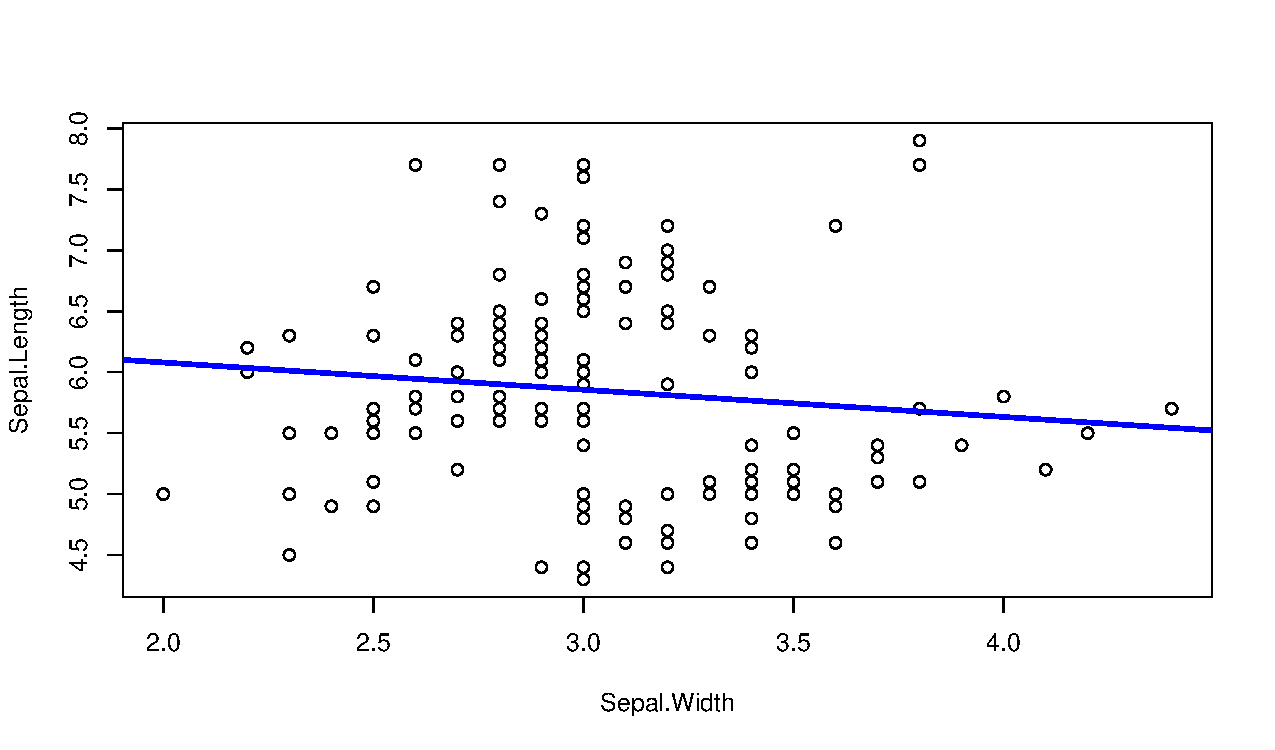
\includegraphics[width=\maxwidth]{figure/iris-Sepal.Length-Sepal.Width-1} 

}


\end{knitrout}

\begin{knitrout}
\definecolor{shadecolor}{rgb}{0.969, 0.969, 0.969}\color{fgcolor}\begin{kframe}
\begin{alltt}
\hldef{SLall} \hlkwb{<-} \hlkwd{lm}\hldef{(Sepal.Length}\hlopt{~}\hldef{.}\hlopt{-}\hldef{Species,}\hlkwc{data}\hldef{=iris)}
\hlkwd{summary}\hldef{(SLall)}
\end{alltt}
\begin{verbatim}
## 
## Call:
## lm(formula = Sepal.Length ~ . - Species, data = iris)
## 
## Residuals:
##      Min       1Q   Median       3Q      Max 
## -0.82816 -0.21989  0.01875  0.19709  0.84570 
## 
## Coefficients:
##              Estimate Std. Error t value Pr(>|t|)    
## (Intercept)   1.85600    0.25078   7.401 9.85e-12 ***
## Sepal.Width   0.65084    0.06665   9.765  < 2e-16 ***
## Petal.Length  0.70913    0.05672  12.502  < 2e-16 ***
## Petal.Width  -0.55648    0.12755  -4.363 2.41e-05 ***
## ---
## Signif. codes:  0 '***' 0.001 '**' 0.01 '*' 0.05 '.' 0.1 ' ' 1
## 
## Residual standard error: 0.3145 on 146 degrees of freedom
## Multiple R-squared:  0.8586,	Adjusted R-squared:  0.8557 
## F-statistic: 295.5 on 3 and 146 DF,  p-value: < 2.2e-16
\end{verbatim}
\end{kframe}
\end{knitrout}

\newpage
\subsubsection*{Decision Tree Classification}

\begin{knitrout}
\definecolor{shadecolor}{rgb}{0.969, 0.969, 0.969}\color{fgcolor}\begin{kframe}
\begin{alltt}
\hlkwd{library}\hldef{(rpart)}
\hlkwd{library}\hldef{(rattle)}
\end{alltt}


{\ttfamily\noindent\bfseries\color{errorcolor}{\#\# Error in `library()`:\\\#\# ! there is no package called 'rattle'}}\begin{alltt}
\hldef{SpeciesClass} \hlkwb{<-} \hlkwd{rpart}\hldef{(Species}\hlopt{~}\hldef{.,}\hlkwc{data}\hldef{=iris)}
\hldef{SpeciesClass}
\end{alltt}
\begin{verbatim}
## n= 150 
## 
## node), split, n, loss, yval, (yprob)
##       * denotes terminal node
## 
## 1) root 150 100 setosa (0.33333333 0.33333333 0.33333333)  
##   2) Petal.Length< 2.45 50   0 setosa (1.00000000 0.00000000 0.00000000) *
##   3) Petal.Length>=2.45 100  50 versicolor (0.00000000 0.50000000 0.50000000)  
##     6) Petal.Width< 1.75 54   5 versicolor (0.00000000 0.90740741 0.09259259) *
##     7) Petal.Width>=1.75 46   1 virginica (0.00000000 0.02173913 0.97826087) *
\end{verbatim}
\begin{alltt}
\hlkwd{fancyRpartPlot}\hldef{(SpeciesClass,}\hlkwc{sub}\hldef{=}\hlsng{""}\hldef{,}\hlkwc{type}\hldef{=}\hlnum{4}\hldef{)}
\end{alltt}


{\ttfamily\noindent\bfseries\color{errorcolor}{\#\# Error in `fancyRpartPlot()`:\\\#\# ! could not find function "{}fancyRpartPlot"{}}}\begin{alltt}
\hlkwd{summary}\hldef{(SpeciesClass)}
\end{alltt}
\begin{verbatim}
## Call:
## rpart(formula = Species ~ ., data = iris)
##   n= 150 
## 
##     CP nsplit rel error xerror       xstd
## 1 0.50      0      1.00   1.17 0.05073460
## 2 0.44      1      0.50   0.70 0.06110101
## 3 0.01      2      0.06   0.10 0.03055050
## 
## Variable importance
##  Petal.Width Petal.Length Sepal.Length  Sepal.Width 
##           34           31           21           14 
## 
## Node number 1: 150 observations,    complexity param=0.5
##   predicted class=setosa      expected loss=0.6666667  P(node) =1
##     class counts:    50    50    50
##    probabilities: 0.333 0.333 0.333 
##   left son=2 (50 obs) right son=3 (100 obs)
##   Primary splits:
##       Petal.Length < 2.45 to the left,  improve=50.00000, (0 missing)
##       Petal.Width  < 0.8  to the left,  improve=50.00000, (0 missing)
##       Sepal.Length < 5.45 to the left,  improve=34.16405, (0 missing)
##       Sepal.Width  < 3.35 to the right, improve=19.03851, (0 missing)
##   Surrogate splits:
##       Petal.Width  < 0.8  to the left,  agree=1.000, adj=1.00, (0 split)
##       Sepal.Length < 5.45 to the left,  agree=0.920, adj=0.76, (0 split)
##       Sepal.Width  < 3.35 to the right, agree=0.833, adj=0.50, (0 split)
## 
## Node number 2: 50 observations
##   predicted class=setosa      expected loss=0  P(node) =0.3333333
##     class counts:    50     0     0
##    probabilities: 1.000 0.000 0.000 
## 
## Node number 3: 100 observations,    complexity param=0.44
##   predicted class=versicolor  expected loss=0.5  P(node) =0.6666667
##     class counts:     0    50    50
##    probabilities: 0.000 0.500 0.500 
##   left son=6 (54 obs) right son=7 (46 obs)
##   Primary splits:
##       Petal.Width  < 1.75 to the left,  improve=38.969400, (0 missing)
##       Petal.Length < 4.75 to the left,  improve=37.353540, (0 missing)
##       Sepal.Length < 6.15 to the left,  improve=10.686870, (0 missing)
##       Sepal.Width  < 2.45 to the left,  improve= 3.555556, (0 missing)
##   Surrogate splits:
##       Petal.Length < 4.75 to the left,  agree=0.91, adj=0.804, (0 split)
##       Sepal.Length < 6.15 to the left,  agree=0.73, adj=0.413, (0 split)
##       Sepal.Width  < 2.95 to the left,  agree=0.67, adj=0.283, (0 split)
## 
## Node number 6: 54 observations
##   predicted class=versicolor  expected loss=0.09259259  P(node) =0.36
##     class counts:     0    49     5
##    probabilities: 0.000 0.907 0.093 
## 
## Node number 7: 46 observations
##   predicted class=virginica   expected loss=0.02173913  P(node) =0.3066667
##     class counts:     0     1    45
##    probabilities: 0.000 0.022 0.978
\end{verbatim}
\end{kframe}
\end{knitrout}

\begin{knitrout}
\definecolor{shadecolor}{rgb}{0.969, 0.969, 0.969}\color{fgcolor}\begin{kframe}
\begin{alltt}
\hldef{titanic}\hlopt{$}\hldef{Class} \hlkwb{<-} \hlkwd{factor}\hldef{(titanic}\hlopt{$}\hldef{Class)}
\end{alltt}


{\ttfamily\noindent\bfseries\color{errorcolor}{\#\# Error:\\\#\# ! object 'titanic' not found}}\begin{alltt}
\hldef{titanic}\hlopt{$}\hldef{Survived} \hlkwb{<-} \hlkwd{factor}\hldef{(titanic}\hlopt{$}\hldef{Survived)}
\end{alltt}


{\ttfamily\noindent\bfseries\color{errorcolor}{\#\# Error:\\\#\# ! object 'titanic' not found}}\begin{alltt}
\hldef{titanic.pass} \hlkwb{<-} \hldef{titanic[titanic}\hlopt{$}\hldef{Class} \hlopt{%in%} \hlkwd{c}\hldef{(}\hlsng{"1st Class"}\hldef{,}\hlsng{"2nd Class"}\hldef{,}\hlsng{"3rd Class"}\hldef{),]}
\end{alltt}


{\ttfamily\noindent\bfseries\color{errorcolor}{\#\# Error:\\\#\# ! object 'titanic' not found}}\begin{alltt}
\hldef{SurvivalModel} \hlkwb{<-} \hlkwd{rpart}\hldef{(Survived}\hlopt{~}\hldef{Sex}\hlopt{+}\hldef{Class}\hlopt{+}\hldef{Age.Whole.Years,}\hlkwc{data}\hldef{=titanic.pass)}
\end{alltt}


{\ttfamily\noindent\bfseries\color{errorcolor}{\#\# Error:\\\#\# ! object 'titanic.pass' not found}}\begin{alltt}
\hldef{SurvivalModel}
\end{alltt}


{\ttfamily\noindent\bfseries\color{errorcolor}{\#\# Error:\\\#\# ! object 'SurvivalModel' not found}}\begin{alltt}
\hlkwd{fancyRpartPlot}\hldef{(SurvivalModel,}\hlkwc{sub}\hldef{=}\hlsng{""}\hldef{,}\hlkwc{type}\hldef{=}\hlnum{4}\hldef{)}
\end{alltt}


{\ttfamily\noindent\bfseries\color{errorcolor}{\#\# Error in `fancyRpartPlot()`:\\\#\# ! could not find function "{}fancyRpartPlot"{}}}\begin{alltt}
\hlkwd{summary}\hldef{(SurvivalModel)}
\end{alltt}


{\ttfamily\noindent\bfseries\color{errorcolor}{\#\# Error:\\\#\# ! object 'SurvivalModel' not found}}\end{kframe}
\end{knitrout}
\end{document}
